\chapter{Analyse von Vier Gewinnt aus spieltheoretischer Sicht}

%Die spieltheoretische Analyse von „Vier Gewinnt“ erfordert eine präzise und formale mathematische Darstellung des Spiels, um dessen strategische Struktur vollständig zu erfassen. Diese Darstellung ermöglicht es, die komplexen Entscheidungsprozesse der Spieler zu analysieren und optimale Strategien zu bestimmen. Im Wesentlichen gibt es zwei zentrale Darstellungsformen, die für die Analyse verwendet werden. Diese Darstellungsformen werden aufgezeigt und bewertet.
%

Die spieltheoretische Analyse des Spiels Vier Gewinnt erfordert eine systematische Untersuchung verschiedener strategischer Komponenten und mathematischer Aspekte. Im Folgenden Kapitel ,,Analyse von Vier Gewinnt aus spieltheoretischer Sicht'' werden die wesentlichen Elemente dieser Analyse detailliert dargestellt.
\section{Darstellung des Spiels in Normalform}
%
%Die Extensivform stellt das Spiel als Spielbaum dar und wird durch den Tupel  beschrieben T= (N,K,P,U,h,p), wobei:
%\begin{itemize}
%	\item N die Menge der Spieler (Spieler 1 und 2)
%	\item K die Menge aller Knoten (Spielpositionen)
%	\item P die Menge der Spielerpositionen
%	\item U die Menge der Endknoten
%	\item h die Auszahlungsfunktion
%	\item p die Vorgängerfunktion ist
%\end{itemize}
%Für Vier Gewinnt ist die Extensivform besonders geeignet, da sie die sequentielle Struktur des Spiels abbildet, die perfekte Information widerspiegelt und eine intuitive Analyse von Zugfolgen ermöglicht.


In der Normalform-Darstellung oder auch Normalform genannt, wird das Spiel als Zwei-Personen-Nullsummenspiel charakterisiert. Das bedeutet, wenn ein Spieler gewinnt ,verliert der andere automatisch . Das Spiel wird in der Normalform rein statisch beschrieben und besteht allgemein aus folgenden Elementen\autocite{gabler_normalform}:
\begin{itemize}
	\item Einer Menge Spieler $(I = {1, ..., i, ..., n})$ 
	\\ Der Wert $I$  gibt die Anzahl der Teilnehmer an.
	
	\item Für jeden Spieler i eine Menge von Strategien $(S_i)$
	\\$(S_i)$ entspricht der Strategiemenge des Spielers$i$, aus dieser er seine Züge wählen kann.
	\item Für jeden Spieler i eine Auszahlungsfunktion/ Nutzenfunktion $(u_i)$
	\\Hierbei wird jeder möglichen Strategiekombination aller Spieler einen reellen Zahlenwert zugeordnet. 
	\\  \begin{align}
		u_i &= \sum S_i \rightarrow \mathbb{R}^{n}  
\end{align}}
\end{itemize}

Ist die Normalform endlich und überschaubar, kann sie auch in einer Matrix dargestellt werden.
Die Matrix muss dabei die verschiedenen Spielsituationen und deren Ausgänge abbilden, wobei jeder Spieler in seiner Zugfolge bis zu sieben verschiedene Strategien pro Zug zur Verfügung hat. Durch die sehr große Anzahl an Strategien ist es nicht mehr überschaubar und daher eher weniger geeignet.
%*************************************************************************************************************************
\section{Komplexität des Spielbaums}
Die Komplexität des Spielbaums ist beträchtlich und wird oft als ,,mittlere Komplexität'' beschrieben. Die liegt daran, dass es eine große Anzahl an möglichen Spielzuständen gibt, aber das Spiel sich dennoch lösbar ist.\\
Die Anzahl der möglichen Konstellationen bei Vier Gewinnt beträgt laut einer Studie von John Tromp 4.531.985.219.092 (circa $4,5*10^{12}$) \autocite{thill2012reinforcement}. Aufgrund dieser enormen Zahl wird deutlich, warum eine vollständige Durchsuchung des Spielbaums für ein Vier-Gewinnt-Spiel eine Herausforderung darstellt.\\
Pro Zug gib es für den Spieler sieben Möglichkeiten. Bereits in der nach ersten Runde hat der Spielbaum $7*7 = 49$ Äste, also 49 mögliche Spielzustände. Das zeigt, dass der Spielbaum trotz der scheinbaren Einfachheit des Spiels Vier Gewinnt, recht komplex ist \autocite{thill2012reinforcement}\autocite{ruile2009viergewinnt}. Aus diesem Grund wurden Ansätze entwickelt, die den Spielbaum mithilfe von verteilten Rechensystemen effizient lösen. Ein Beispiel hierfür ist ,,Shard Solver'' \autocite{yokota2022exploration}.

% Der Verzweigungsfaktor wird durch die sieben möglichen Züge pro Spielsituation bestimmt, wobei sich die Komplexität mit jeder Erhöhung der Baumtiefe multipliziert2
%. Die computationellen Herausforderungen ergeben sich aus der Notwendigkeit, große Mengen von Spielzuständen zu analysieren und zu bewerten. Dabei müssen bestimmte Verhaltensregeln der Spieler berücksichtigt werden, wie etwa das sofortige Nutzen von Gewinnmöglichkeiten und das Verhindern gegnerischer Gewinnzüge2
%. Die Analyse zeigt, dass trotz der scheinbaren Einfachheit der Spielregeln eine erhebliche mathematische Komplexität vorliegt. Die praktische Implementierung optimaler Strategien erfordert daher sowohl theoretisches Verständnis als auch effiziente Algorithmen zur Bewältigung des großen Zustandsraums. Besonders die Kontrolle strategisch wichtiger Positionen und die Fähigkeit, mehrere Züge vorauszudenken, sind entscheidend für den Spielerfolg2
.
\begin{figure}[H]
	\centering
	\includegraphics[width=0.9\linewidth]{"images/Baum1"}
	\caption[Spielbaum nach der 2. Tiefe]{Spielbaum nach dem 1. Zug von Spieler 1}
	\label{fig:baum1}
\end{figure}

\begin{figure}[H]
	\centering
	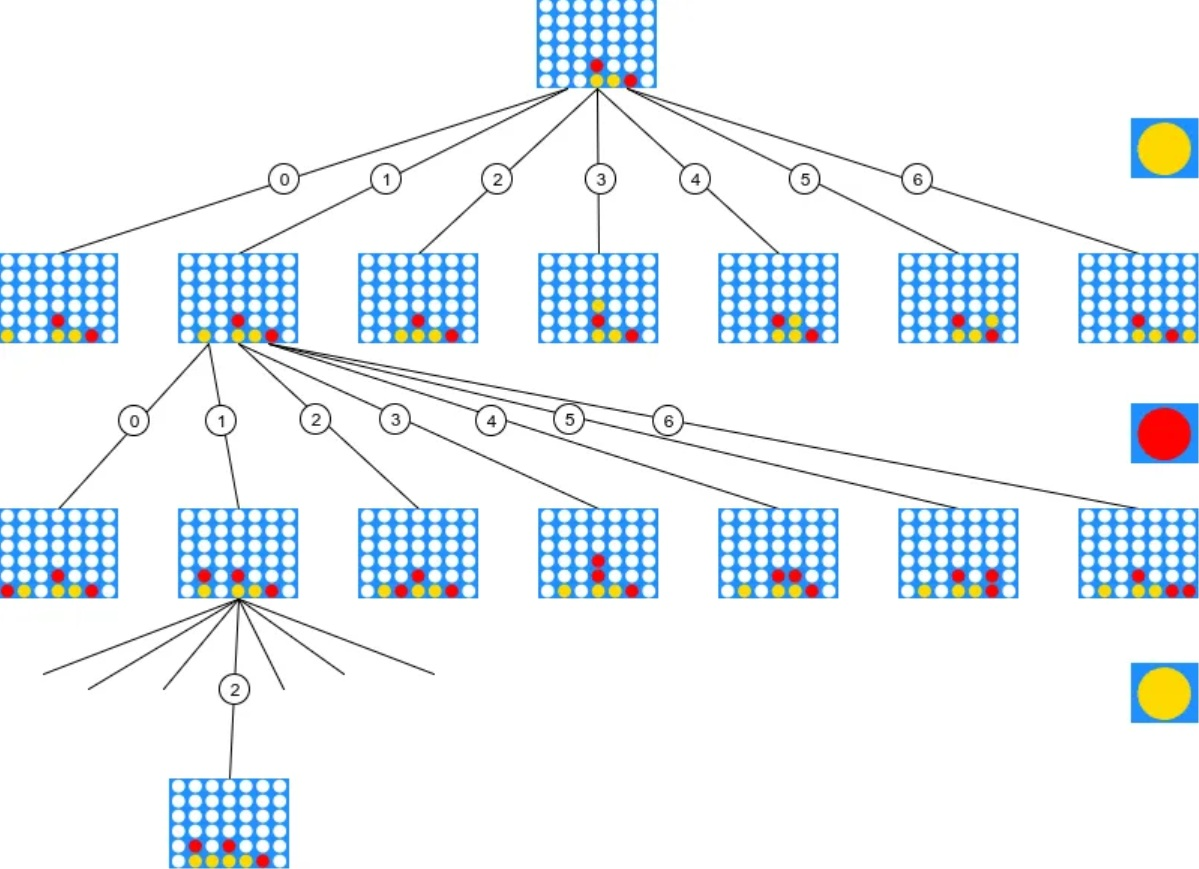
\includegraphics[width=0.9\linewidth]{"images/Baum2}
	\caption[Spielbaum nach dem 4. Zug. Quelle: \cite{vandewiele2017}]{Schematische Darstellung des Spielbaum nach dem 4. bis zum 7. Zug}
	\label{fig:Baum2}
\end{figure}



 \section{Darstellung des Spiels in Extensivform}
%Die Normalform hingegen repräsentiert das Spiel als Matrix G=(N,S,u) , mit:
%\begin{itemize}
%	\item N als Menge der Spieler
%	\item S als Menge der Strategieprofile
%	\item u als Auszahlungsfunktion
%\end{itemize}
%
%Die mathematische Beschreibung des Spielbaums erfolgt durch:
%T = (V,E,v_0) 
%wobei:
%\begin{itemize}
%	\item V die Menge aller Knoten
%	\item E die Menge der Kanten (mögliche Züge)
%	\item v_0 der Wurzelknoten (Ausgangsposition) ist
%\end{itemize}
%
%Die Darstellung in Normalform ist aufgrund der hohen Anzahl möglicher Strategien sehr umfangreich und für praktische Analysen weniger geeignet. Die Größe der Normalform-Matrix wächst exponentiell mit der Spieltiefe.

%*******Noch Ändern************************************************************************************
%Der Spielbaum in der Extensivform zeigt die sequentielle Struktur des Spiels. Jeder Knoten repräsentiert eine Spielsituation, von der aus verschiedene Zugmöglichkeiten ausgehen. Die Teilspielanalyse ermöglicht es, einzelne Spielsituationen isoliert zu betrachten und optimale Strategien zu entwickeln5
%. Bei perfektem Spiel beider Spieler ergeben sich dabei klare Strukturen, die durch den Zermelo'schen Bestimmtheitssatz beschrieben werden können

Die Extensivform Darstellung ist eine aufschlussreiche Methode.
Sie ermöglicht eine detaillierte Abbildung des Spielverlaufs und der Entscheidungsmöglichkeiten aller Spieler.
In dieser Form wird ein Spielbaum verwendet, der aus Knoten und Kanten besteht \autocite{einsiedler2014spieltheorie}. 
Der Baum beginnt mit einem Wurzelknoten hier ist es ein Leeres Spielfeld mit 42 freien Feldern. Die Verbindungen zwischen den Knoten, auch Kanten genannt, stellen die möglichen Züge für den Spieler da. Die Knoten, an denen die Kanten zusammen laufen repräsentieren eine Entscheidung eines Spieler. Die Endknoten zeigen die möglichen Ausgänge für das Spiel an.
Bei vier gewinnt stellt jeden Ebene des Spielbaums ein Spielzug da. Pro Zug gibt es immer sieben Möglichkeiten den Spielstein zu platzieren. Das Bedeutet, von jedem Knoten gehen sieben Kanten weg. Allerdings ist der Baum durch die Spielfeldgröße auf 42 mögliche Züge begrenzt.\\
Um die Extensivform praktisch nutzen zu können, werden Vereinfachungen und Optimierungen durchgeführt.

\section{Strategien und Gleichgewichte}
%*******Noch Ändern************************************************************************************
Die Analyse der Strategien zeigt, dass es im Vier Gewinnt dominante Strategien gibt. Nach dem Zermelo'schen Bestimmtheitssatz lässt sich das Spiel in eine von drei Kategorien einordnen, wobei sich herausgestellt hat, dass der erste Spieler eine dominante Strategie besitzt5
. Die Nash-Gleichgewichte manifestieren sich in den optimalen Zugfolgen, wobei die Kontrolle der zentralen Spalten eine entscheidende Rolle spielt2
.


	